%%%%%%%%%%%%%%%%%%%%%%%%%%%%%%%%%%%%%%%%%%%%%%%%%%
\frame
{
\frametitle{So far}

The resampling methods are:
\begin{itemize}
\item Bootstrap \textbf{re}sampling: generate samples with the same size $n$ as $\mathbf{x}$  with replacement.

\

\item Jackknife \textbf{sub}sampling : generate samples with a smaller size  than $\mathbf{x}$  without replacement.
\end{itemize}

Used for:
\begin{itemize}
\item Compute accuracy measures (standard error, bias, etc.) of a statistic $\hat{\theta}$ from one set $\mathbf{x}=(x_1,\cdots,x_n)$.

\item Compare two sets of observations:  the example of the mouse data
\end{itemize} 

}
%%%%%%%%%%%%%%%%%%%%%%%%%%%%%%%%%%%%%%%%%%%%%%%%%%
\frame
{
\frametitle{Example on the mouse data}

\begin{table}[!h]
\begin{tabular}{|c|c|}
\hline
&\\
 Data (Treatment group) & 94; 197; 16; 38; 99; 141; 23 \\
&\\
\hline
& \\
Data (Control group) & 52; 104; 146; 10; 51; 30; 40; 27; 46 \\
& \\
\hline
\end{tabular}
\caption{The mouse data [Efron]. 16 mice  assigned to a treatment group (7) or a control group (9). Survival in days following a test surgery.  }
\end{table}

\centering{\alert{\textbf{Did the treatment prolong survival ?}}}


}


%%%%%%%%%%%%%%%%%%%%%%%%%%%%%%%%%%%%%%%%%%%%%%%%%
\frame
{
\frametitle{Example on the mouse data}


\begin{enumerate}
\item  Compute $B$ bootstrap samples for each group

\

\begin{itemize}
\item  $\mathbf{x}_{Treat}^{*(b)}=(x_{Treat\ 1}^{*(b)},\cdots,x_{Treat\ 7}^{*(b)})$ 

\

\item $\mathbf{x}_{Cont}^{*(b)}=(x_{Cont\ 1}^{*(b)},\cdots,x_{Cont\ 9}^{*(b)})$
\end{itemize}

\

\item $B$ bootstrap replications are computed: $\hat{\theta}^{*}(b)=\overline{x}^{*(b)}_{Treat}-\overline{x}^{*(b)}_{Cont}$

\

\item you can approximate the p.d.f. of the replications by a histogram.  

\end{enumerate}

}
%%%%%%%%%%%%%%%%%%%%%%%%%%%%%%%%%%%%%%%%%%%%%%%%%%
\frame
{
\frametitle{Example on the mouse data}

\begin{figure}
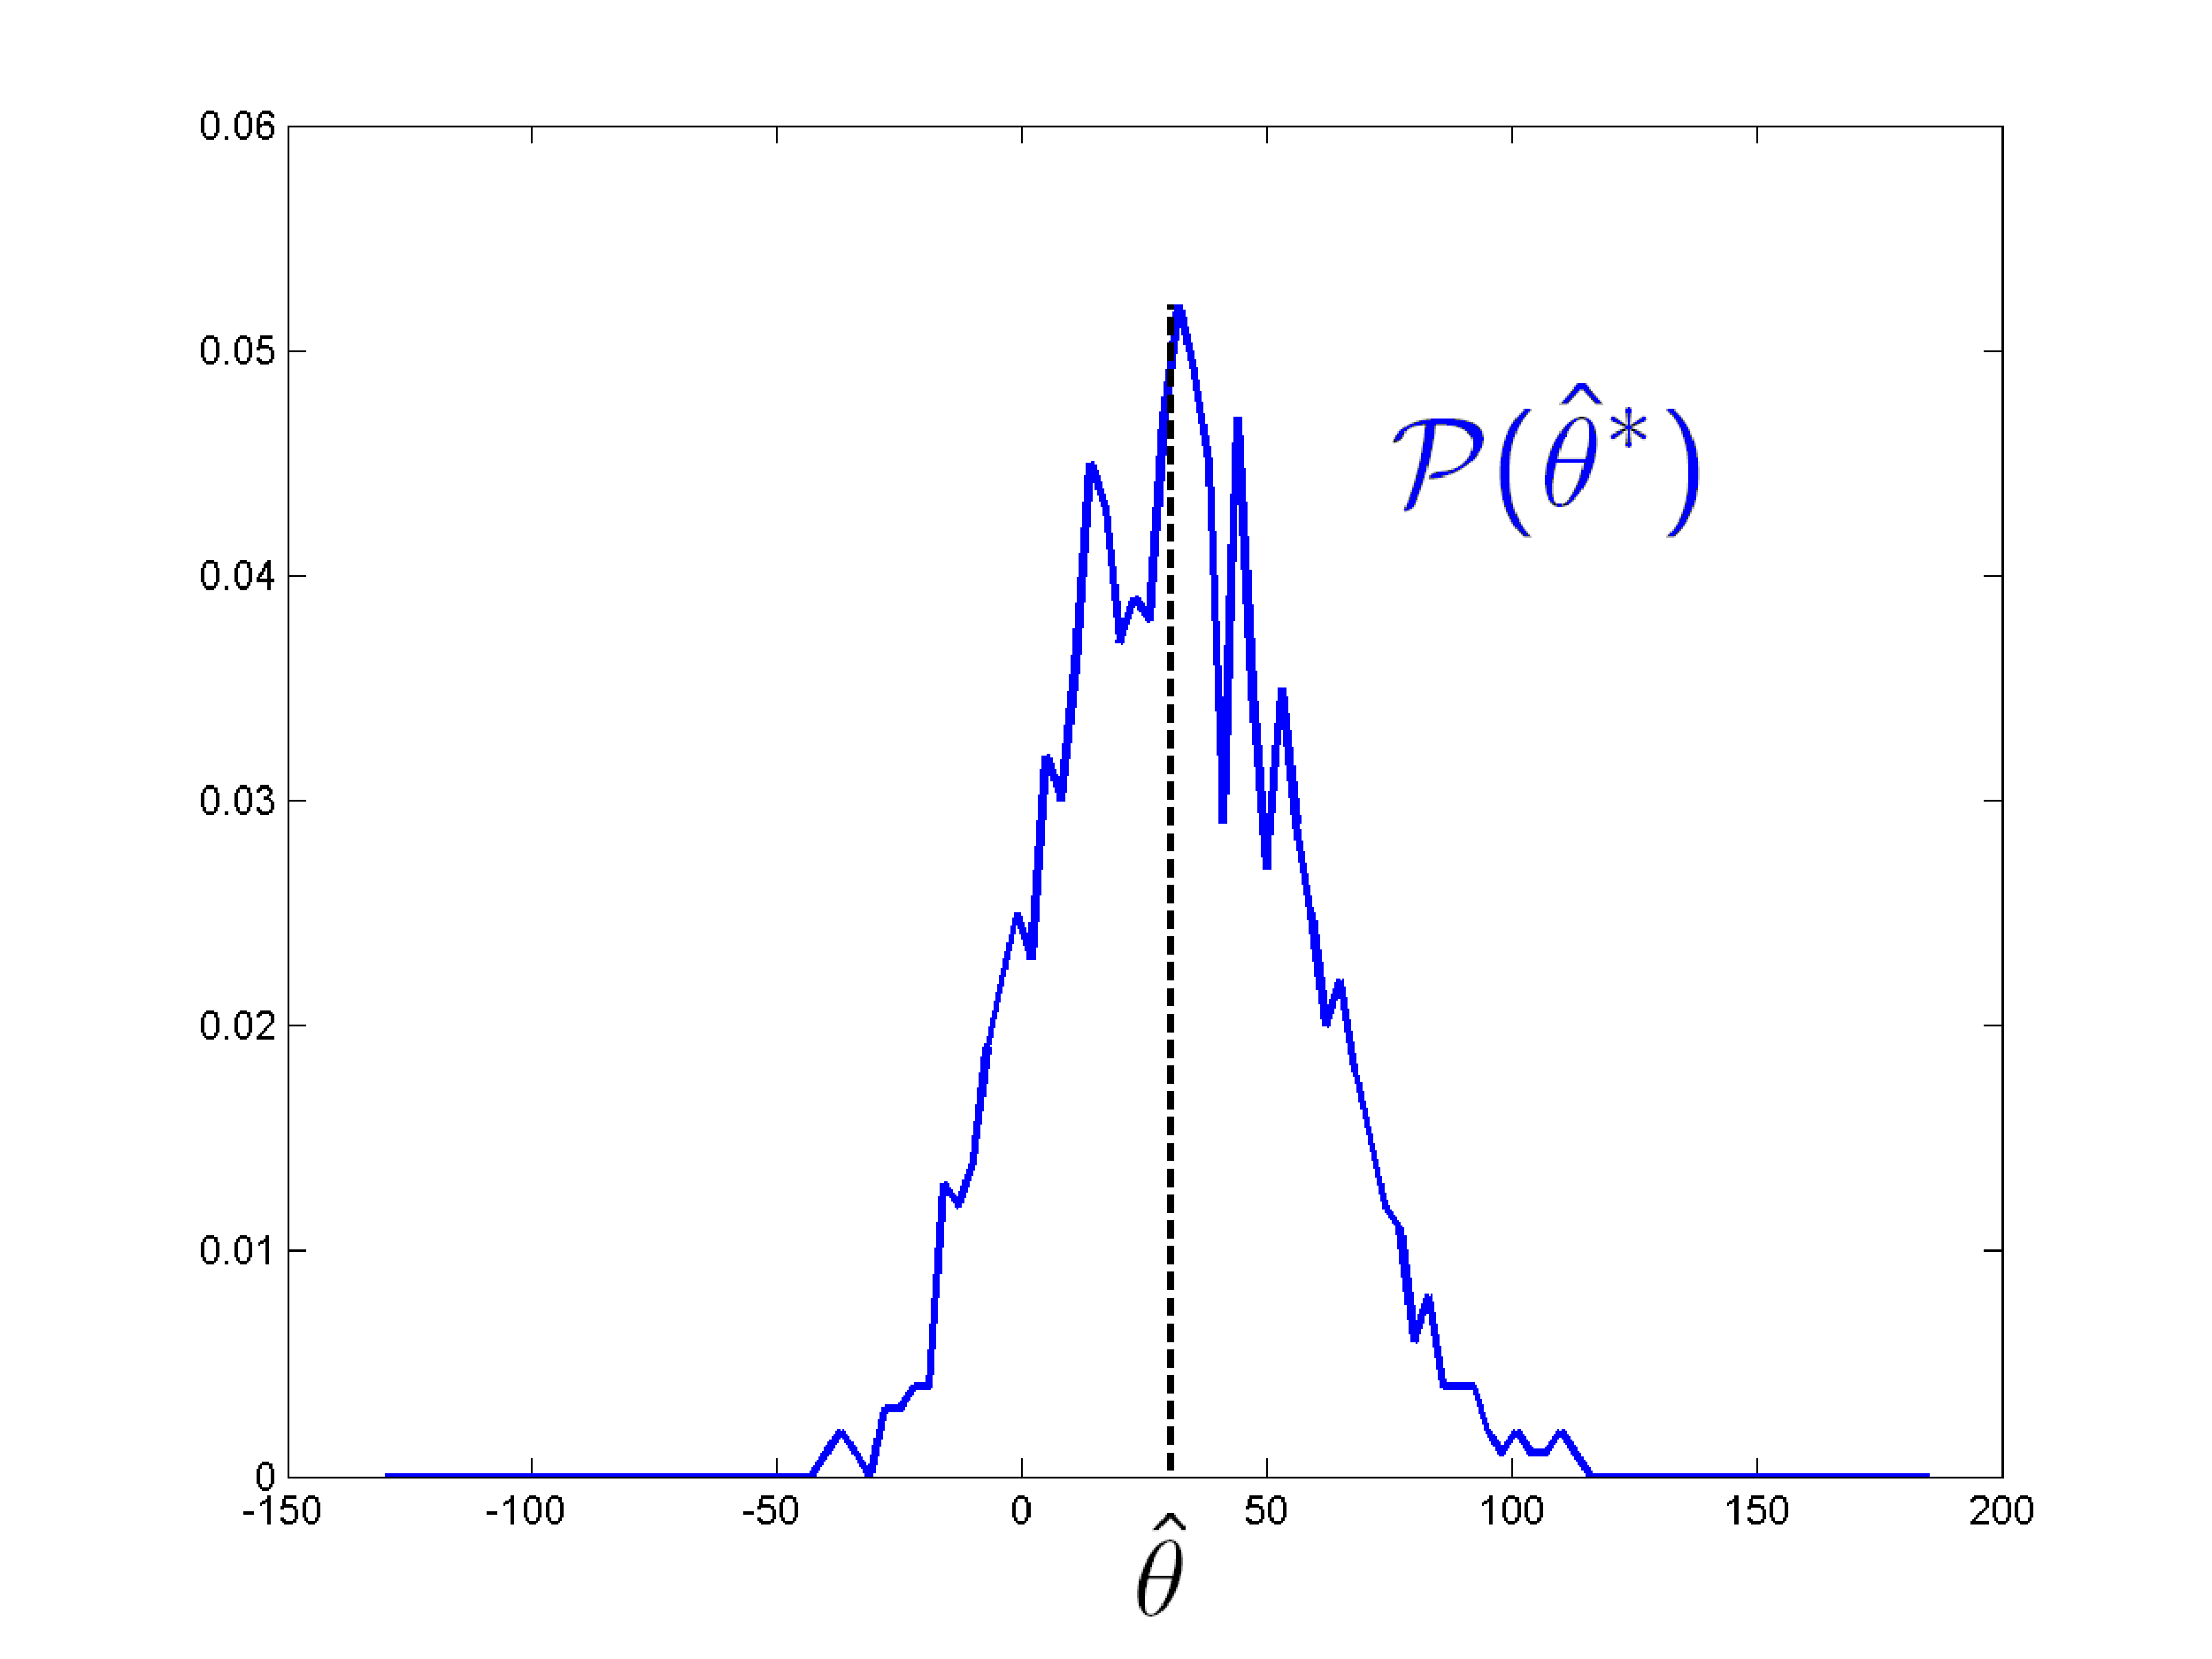
\includegraphics[scale=.2]{originalboot}
\caption{P.d.f. $\mathcal{P}(\hat{\theta}^{*})$ (histogram)  of the replication $\hat{\theta}^{*}$ ( $\hat{\theta}=30.63$
and $\hat{se}_B=26.85$).}
\end{figure}

}
%%%%%%%%%%%%%%%%%%%%%%%%%%%%%%%%%%%%%%%%%%%%%%%%%%
%\frame
%{
%\frametitle{Example on the mouse data}

%\begin{figure}
%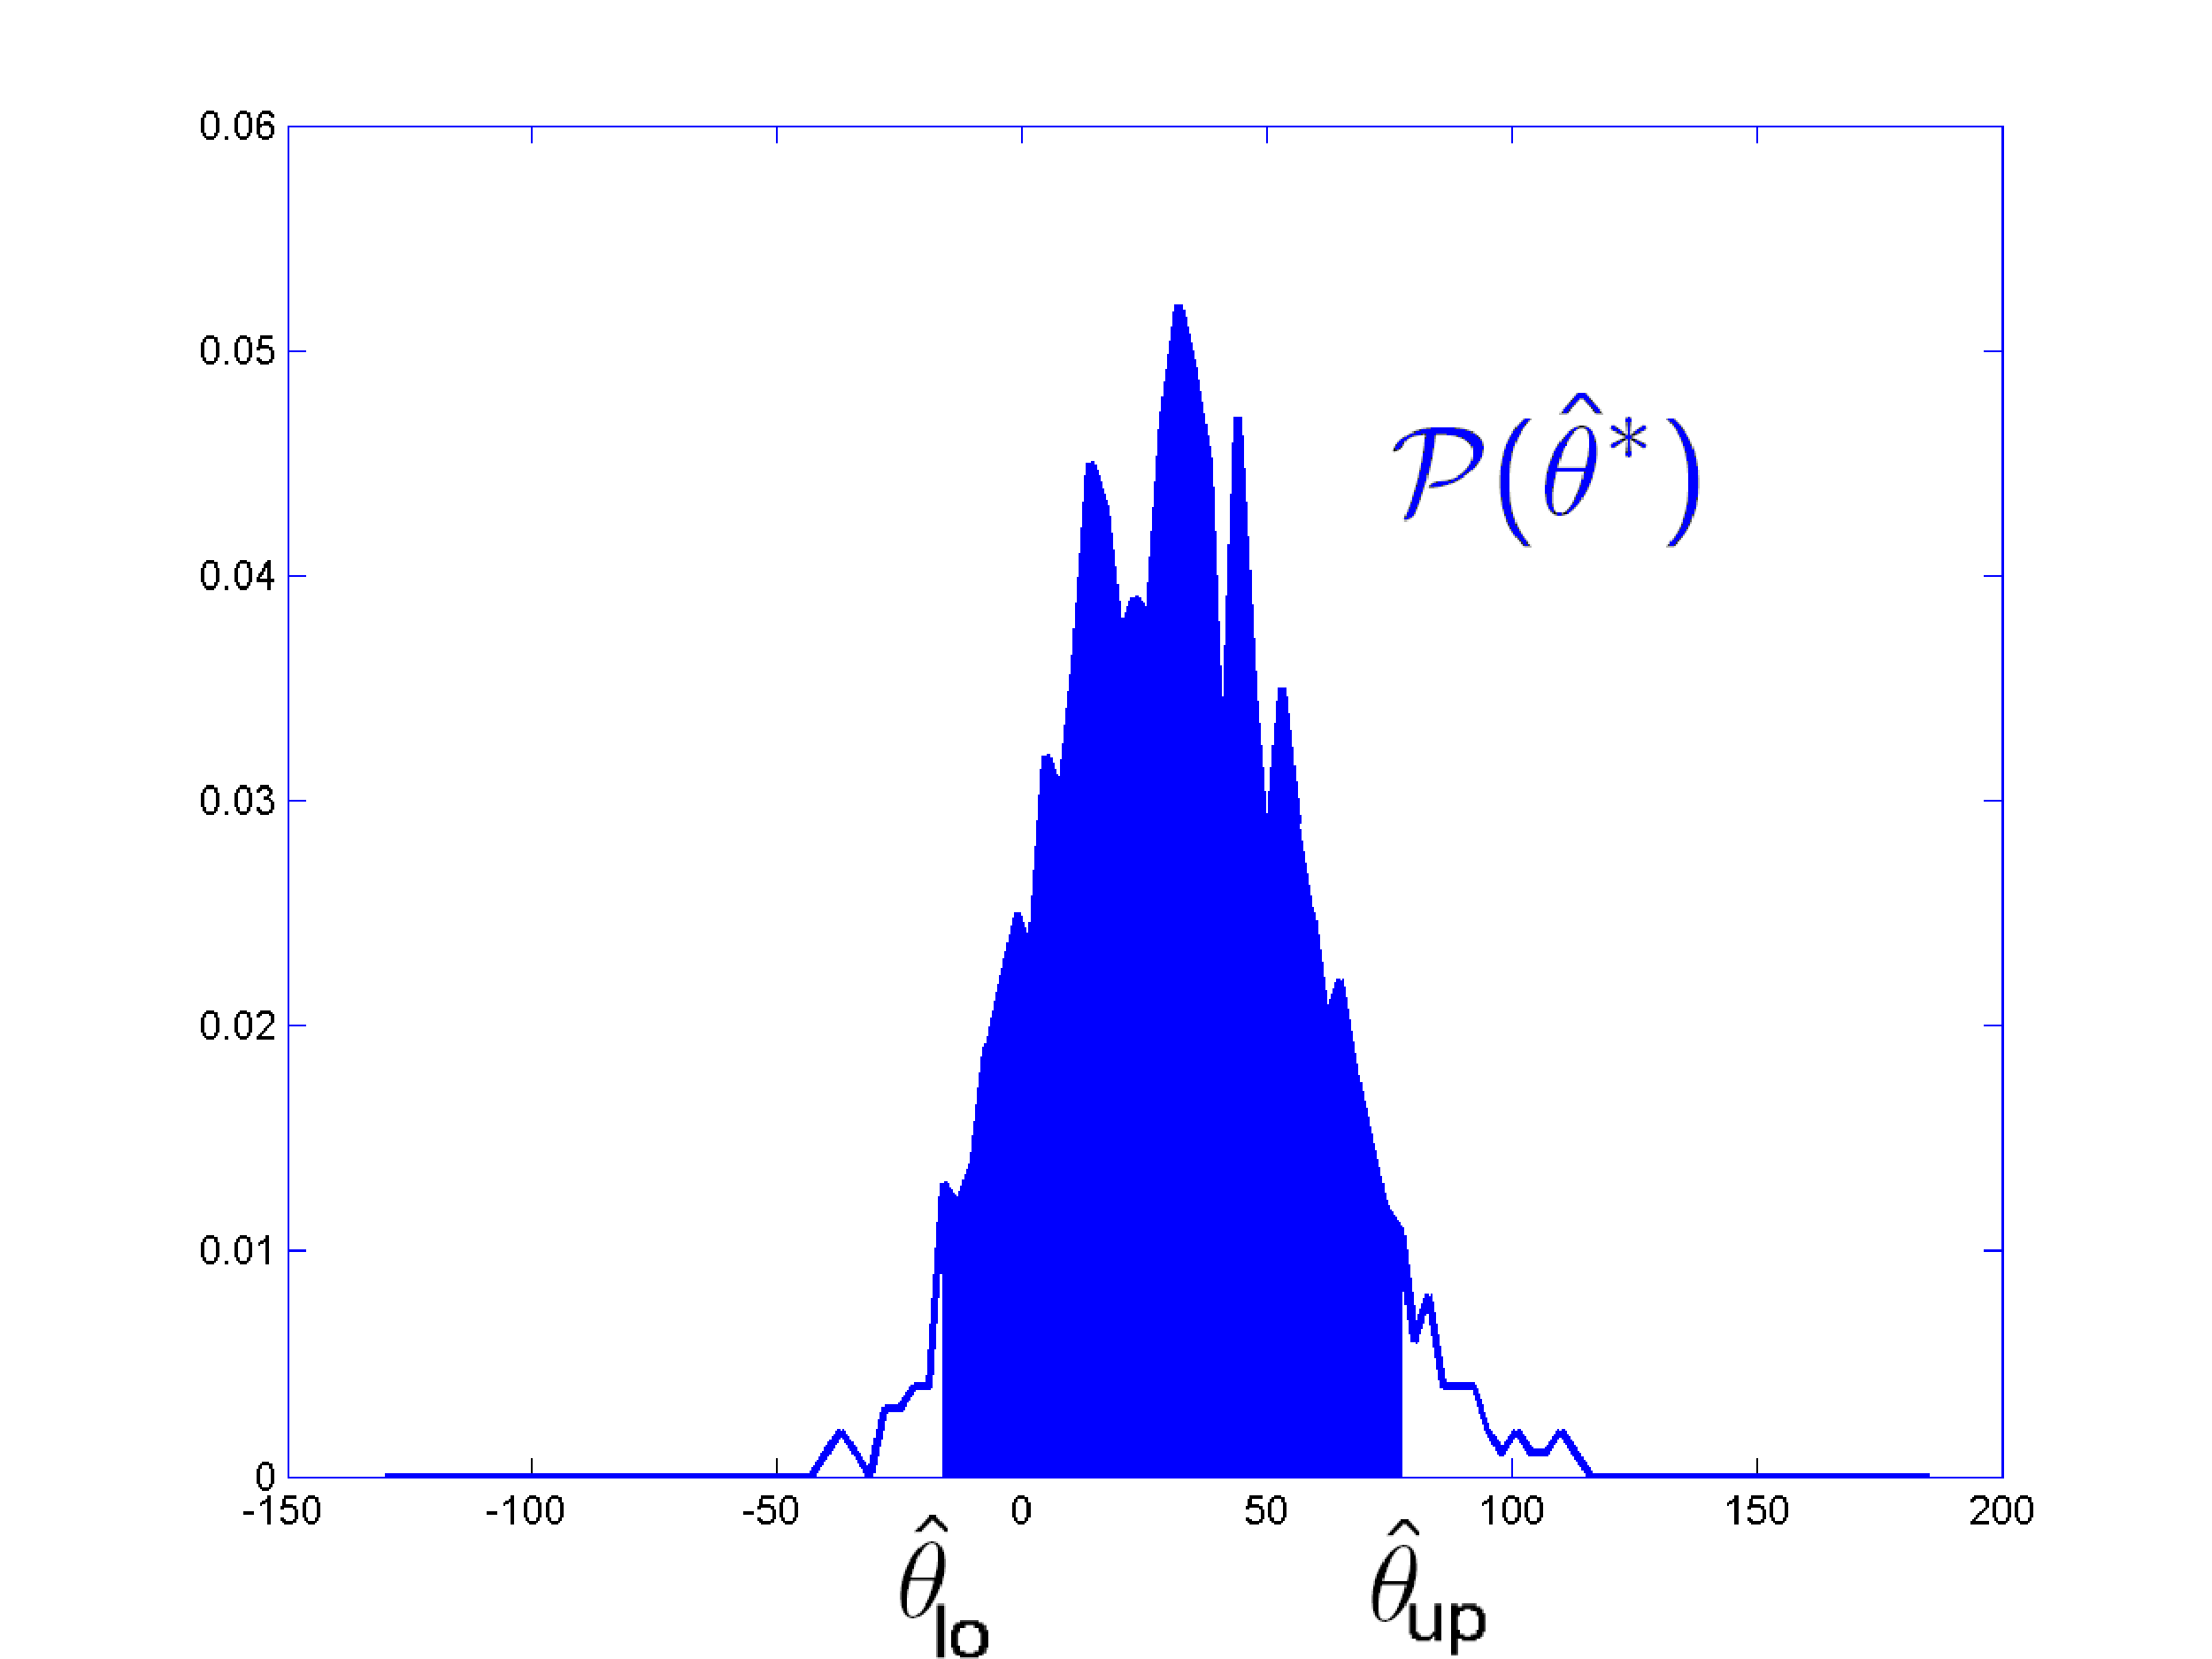
\includegraphics[scale=.2]{originalboot2}
%\caption{P.d.f. (histogram) of the replication $\hat{\theta}$ ($\mathcal{P}(\hat{\theta}^{*})$) with the 90 \% confidence interval defined by $\hat{\theta}_{lo}=\hat{\theta}-1.645*\hat{se}$ and $\hat{\theta}_{up}=\hat{\theta}+1.645*\hat{se}$. }
%\end{figure}
%}
\frame{
\frametitle{Introduction}

\begin{itemize}
\item Two sample problem : definitions

\

\item Parametric solution

\

\item Non parametric solution:

\

\begin{itemize}
\item permutation test

\

\item randomization test

\

\item bootstrap test
\end{itemize}
\end{itemize}
}
%%%%%%%%%%%%%%%%%%%%%%%%%%%%%%%%%%%%%%%%%%%%%%%%%%
\frame
{
\frametitle{The two sample problem}

Two independent random sample are observed $\mathbf{x}_{a}$ and $\mathbf{x}_{b}$ drawn from possibly different probability density functions:
$$
\begin{array}{l}
 f_{a}  \rightsquigarrow \mathbf{x}_a=\lbrace x_{a,1},\cdots, x_{a,n} \rbrace\\
\\
f_{b}  \rightsquigarrow \mathbf{x}_b=\lbrace x_{b,1},\cdots, x_{b,m} \rbrace
\end{array}
$$
\begin{definition}
The \alert{null hypothesis $\mathcal{H}_0$} assumes that there is no difference in between the density function $f_a=f_b$.
\end{definition}

}


%%%%%%%%%%%%%%%%%%%%%%%%%%%%%%%%%%%%%%%%%%%%%%%%
\frame
{
\frametitle{Hypothesis  test and Achieved significance level (ASL)}

\begin{definition}
A \alert{hypothesis test} is a way of deciding whether or not the data decisively reject the hypothesis $\mathcal{H}_0$. 
\end{definition}

\begin{definition}
The \alert{achieved significance level} of the test (ASL) is defined as:
$$
\begin{array}{ll}
\mathrm{ASL}&= \pmb{\mathcal{P}}(\hat{\theta}^{*}\geq \hat{\theta}|\mathcal{H}_0)\\
&\\
&=\int^{+\infty}_{\hat{\theta}} \mathcal{P}(\hat{\theta}^{*}|\mathcal{H}_0) \ d\hat{\theta}^{*}\\
\end{array}
$$ 
The smaller ASL, the stronger is the evidence of  $\mathcal{H}_0$ false. The notation star differentiates between  an hypothetical value $\hat{\theta}^{*}$ generated according to $\mathcal{H}_0$, and the actual observation $\hat{\theta}$.
\end{definition}
}
%%%%%%%%%%%%%%%%%%%%%%%%%%%%%%%%%%%%%%%%%%%%%%%%%%
\frame
{
\frametitle{Parametric test}

\begin{itemize}

\item A tradionnal way is to consider some hypotheses: $f_a \sim \mathcal{N}(\mu_a, \sigma^2)$ and $f_b \sim \mathcal{N}(\mu_b, \sigma^2)$, and the null hypothesis becomes $\mu_a=\mu_b$. 

\

\item Under $\mathcal{H}_{0}$, the statistic $\hat{\theta}=\overline{x}_a-\overline{x}_b$ can be modelled as a normal distribution with mean 0 and variance $\sigma^2_{\hat{\theta}}=\sigma^2 (\frac{1}{m}+\frac{1}{n})$. 

\

\item The ASL is then computed:
$$
\mathrm{ASL}= \int^{+\infty}_{\hat{\theta}} 
\frac{
e^{ \frac{- (\hat{\theta}^{*}-\hat{\theta} )^{2} } {2\sigma^2_{\hat{\theta}}  }}} {\sqrt{2\pi} \sigma_{\hat{\theta}}} \ 
d\hat{\theta}^{*}
$$

\end{itemize}
}
%%%%%%%%%%%%%%%%%%%%%%%%%%%%%%%%%%%%%%%%%%%%%%%%%%
\frame
{
\frametitle{Parametric test}

\begin{itemize}
\item $\sigma$ is unknown and has to be estimated from the data:
$$ 
\overline{\sigma}^2= \frac{\sum_{i=1}^{n} (x_{ai}-\overline{x}_{a})^2 +\sum_{i=1}^{m} (x_{bi}-\overline{x}_{b})^2} {m+n-2}
$$



\item For the mouse data $\mathrm{ASL}=.131$ : the null hypothesis cannot be rejected.

\

\item However, this (parametric) method relies on the hypotheses made while calculating the ASL.  

\end{itemize} 

}
%%%%%%%%%%%%%%%%%%%%%%%%%%%%%%%%%%%%%%%%%%%%%%%%%%
\frame
{
\frametitle{Permutation tests}

\begin{itemize}
\item \textit{Permutation tests} are a computer-intensive statistical technique that predates computers. 

\ 

\item This idea was introduced by R.A. Fisher in the 1930's.

\

\item The main application of permutation tests is the two-sample problem. 

\end{itemize}
}




%%%%%%%%%%%%%%%%%%%%%%%%%%%%%%%%%%%%%%%%%%%%%%%%%
\frame
{
\frametitle{Computation of the two sample permutation test statistic}

\begin{block}{}
Notation $m$ number of values in  observation $\mathbf{x}_{Treat}$, $n$ number of values in observation $\mathbf{x}_{Cont}$. 

\alert{If $\mathcal{H}_0$ is true, then:} 
\begin{enumerate}
\item We can combine the values from both observations in one of size $m+n=N$:  $\mathbf{x}=\lbrace \mathbf{x}_{Treat}, \mathbf{x}_{Cont}\rbrace$.

\

\item Take a subsample $\mathbf{x}_{Treat}^{*}$ from $\mathbf{x}$ of size $m$. The remaining $n$ values constitute the subsample $\mathbf{x}_{Cont}^{*}$.

\

\item Compute the replication $\overline{x}^{*}_{Treat}$ and $\overline{x}^{*}_{Cont}$ on $\mathbf{x}_{Treat}^{*}$ and $\mathbf{x}_{Cont}^{*}$ respectively.

\

\item Compute the replication of the difference $\hat{\theta}^{*}=\overline{x}^{*}_{Treat}-\overline{x}^{*}_{Cont}$.
\end{enumerate}
\end{block}
}
%%%%%%%%%%%%%%%%%%%%%%%%%%%%%%%%%%%%%%%%%%%%%%%%%
\frame
{
\frametitle{Example on the mouse data}

\begin{figure}[!h]
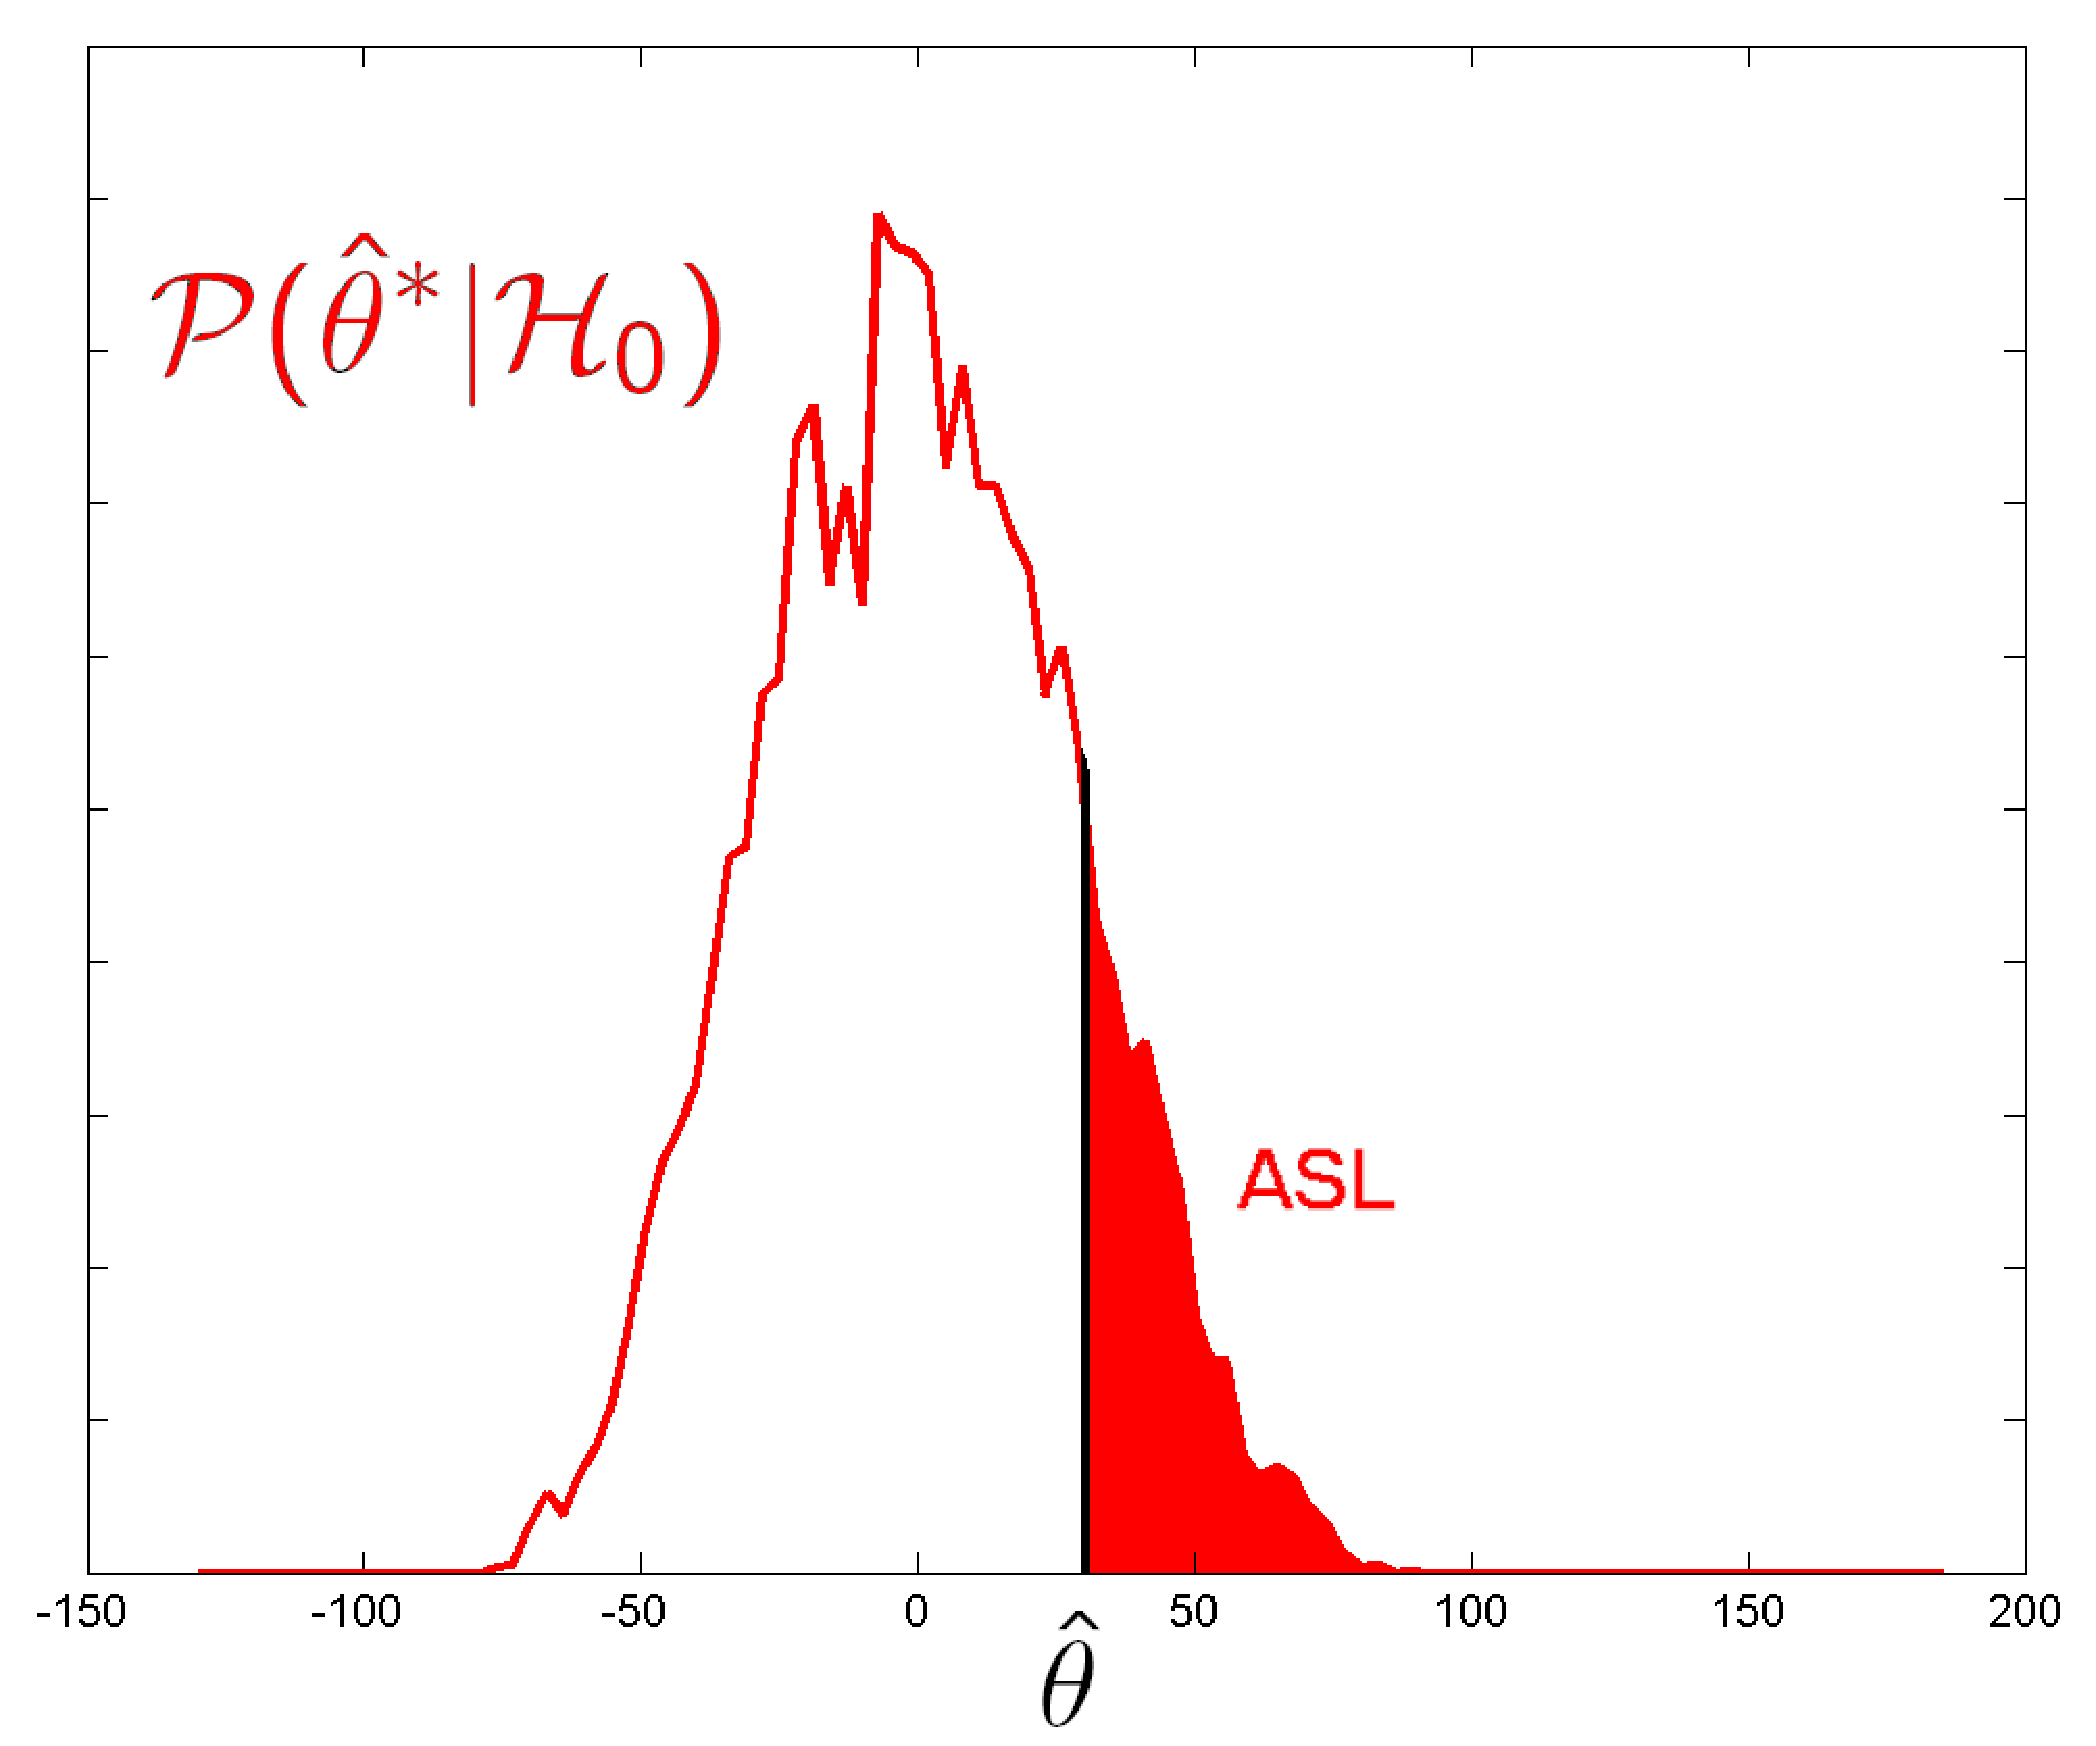
\includegraphics[scale=.15]{perm}
\caption{Histogram of the permutation replications $\mathcal{P}(\hat{\theta}^{*}|\mathcal{H}_{0})$. ASL is the red surface ($\mathrm{ASL}_{perm}=0.14$).}
\end{figure}

\begin{block}{}
\small{If the original difference $\hat{\theta}=d=\overline{x}_{Treat}-\overline{x}_{Cont}$ falls outside the 95\% of the distribution of the permutation replication  (i.e. $\mathrm{ASL}_{perm}<0.05$), then the null hypothesis is rejected.}  
\end{block}
}
%%%%%%%%%%%%%%%%%%%%%%%%%%%%%%%%%%%%%%%%%%%%%%%%%
\frame
{
\frametitle{Computation of the two sample permutation test statistic}

\begin{beamercolorbox}[wd=\linewidth, rounded=true,shadow=true]{postit}

\begin{enumerate}
\item $\mathbf{x}=\lbrace \mathbf{x}_a;\mathbf{x}_b \rbrace$ of size $n+m=N$. 

\

\item Compute  all  :


\begin{itemize}
\item $
\left(
\begin{array}{l}
 N\\ 
 n \\
 \end{array}
\right)
$ permutation samples $\mathbf{x}^{*}$. Select the $n$ first values to define $\mathbf{x}^{*}_a$ and the last $m$ ones to define $\mathbf{x}^{*}_b$

\ 

\item  $
\left(
\begin{array}{l}
 N\\ 
 n \\
 \end{array}
\right)
$ replications $\hat{\theta}^{*}(b)=\overline{x}_{a}^{*}-\overline{x}_{b}^{*}$
\end{itemize}

\

\item Approximate $\mathrm{ASL}_{perm}$ by:
$$
\widehat{\mathrm{ASL}}_{perm}= \frac{\# \lbrace \hat{\theta}^{*} \geq \hat{\theta} \rbrace}{\left(
\begin{array}{l}
 N\\ 
 n \\
 \end{array}
\right)}
$$
\end{enumerate}

\end{beamercolorbox}
}
%%%%%%%%%%%%%%%%%%%%%%%%%%%%%%%%%%%%%%%%%%%%%%%%
\frame{
\frametitle{Remark on the permutation test}
\begin{itemize}
\item The histogram of the \alert{permutation replications} $\hat{\theta}^{*}$ approximates $\mathcal{P}(\hat{\theta}^*|\mathcal{H}_0)$.

\

\item The resamples are not really permutations but more combinations. 
  
\

\item $\left(
\begin{array}{l}
 N\\ 
 n \\
 \end{array}
\right)$  can be huge so in practice, ASL$_{perm}$ is approximated by Monte Carlo methods. 

\end{itemize}
}
%%%%%%%%%%%%%%%%%%%%%%%%%%%%%%%%%%%%%%%%%%%%%%%%%
\frame
{
\frametitle{Computation of the two sample randomization test statistic}

\begin{beamercolorbox}[wd=\linewidth, rounded=true,shadow=true]{postit}

\begin{enumerate}
\item $\mathbf{x}=\lbrace \mathbf{x}_a;\mathbf{x}_b \rbrace$ of size $n+m=N$. 

\

\item Compute $B$ times:


\begin{itemize}
\item Randomly selected permutation samples $\mathbf{x}^{*}$. Select the $n$ first values to define $\mathbf{x}^{*}_a$ and the last $m$ ones to define $\mathbf{x}^{*}_b$

\ 

\item Compute the replications $\hat{\theta}^{*}(b)=\overline{x}_{a}^{*}-\overline{x}_{b}^{*}$
\end{itemize}

\

\item Approximate $\mathrm{ASL}_{perm}$ by:
$$
\widehat{\mathrm{ASL}}_{perm}= \frac{\# \lbrace \hat{\theta}^{*} \geq \hat{\theta} \rbrace}{B}
$$
\end{enumerate}

\end{beamercolorbox}
}
%%%%%%%%%%%%%%%%%%%%%%%%%%%%%%%%%%%%%%%%%%%%%%
\frame
{
\frametitle{Remarks}

\begin{figure}[!h]
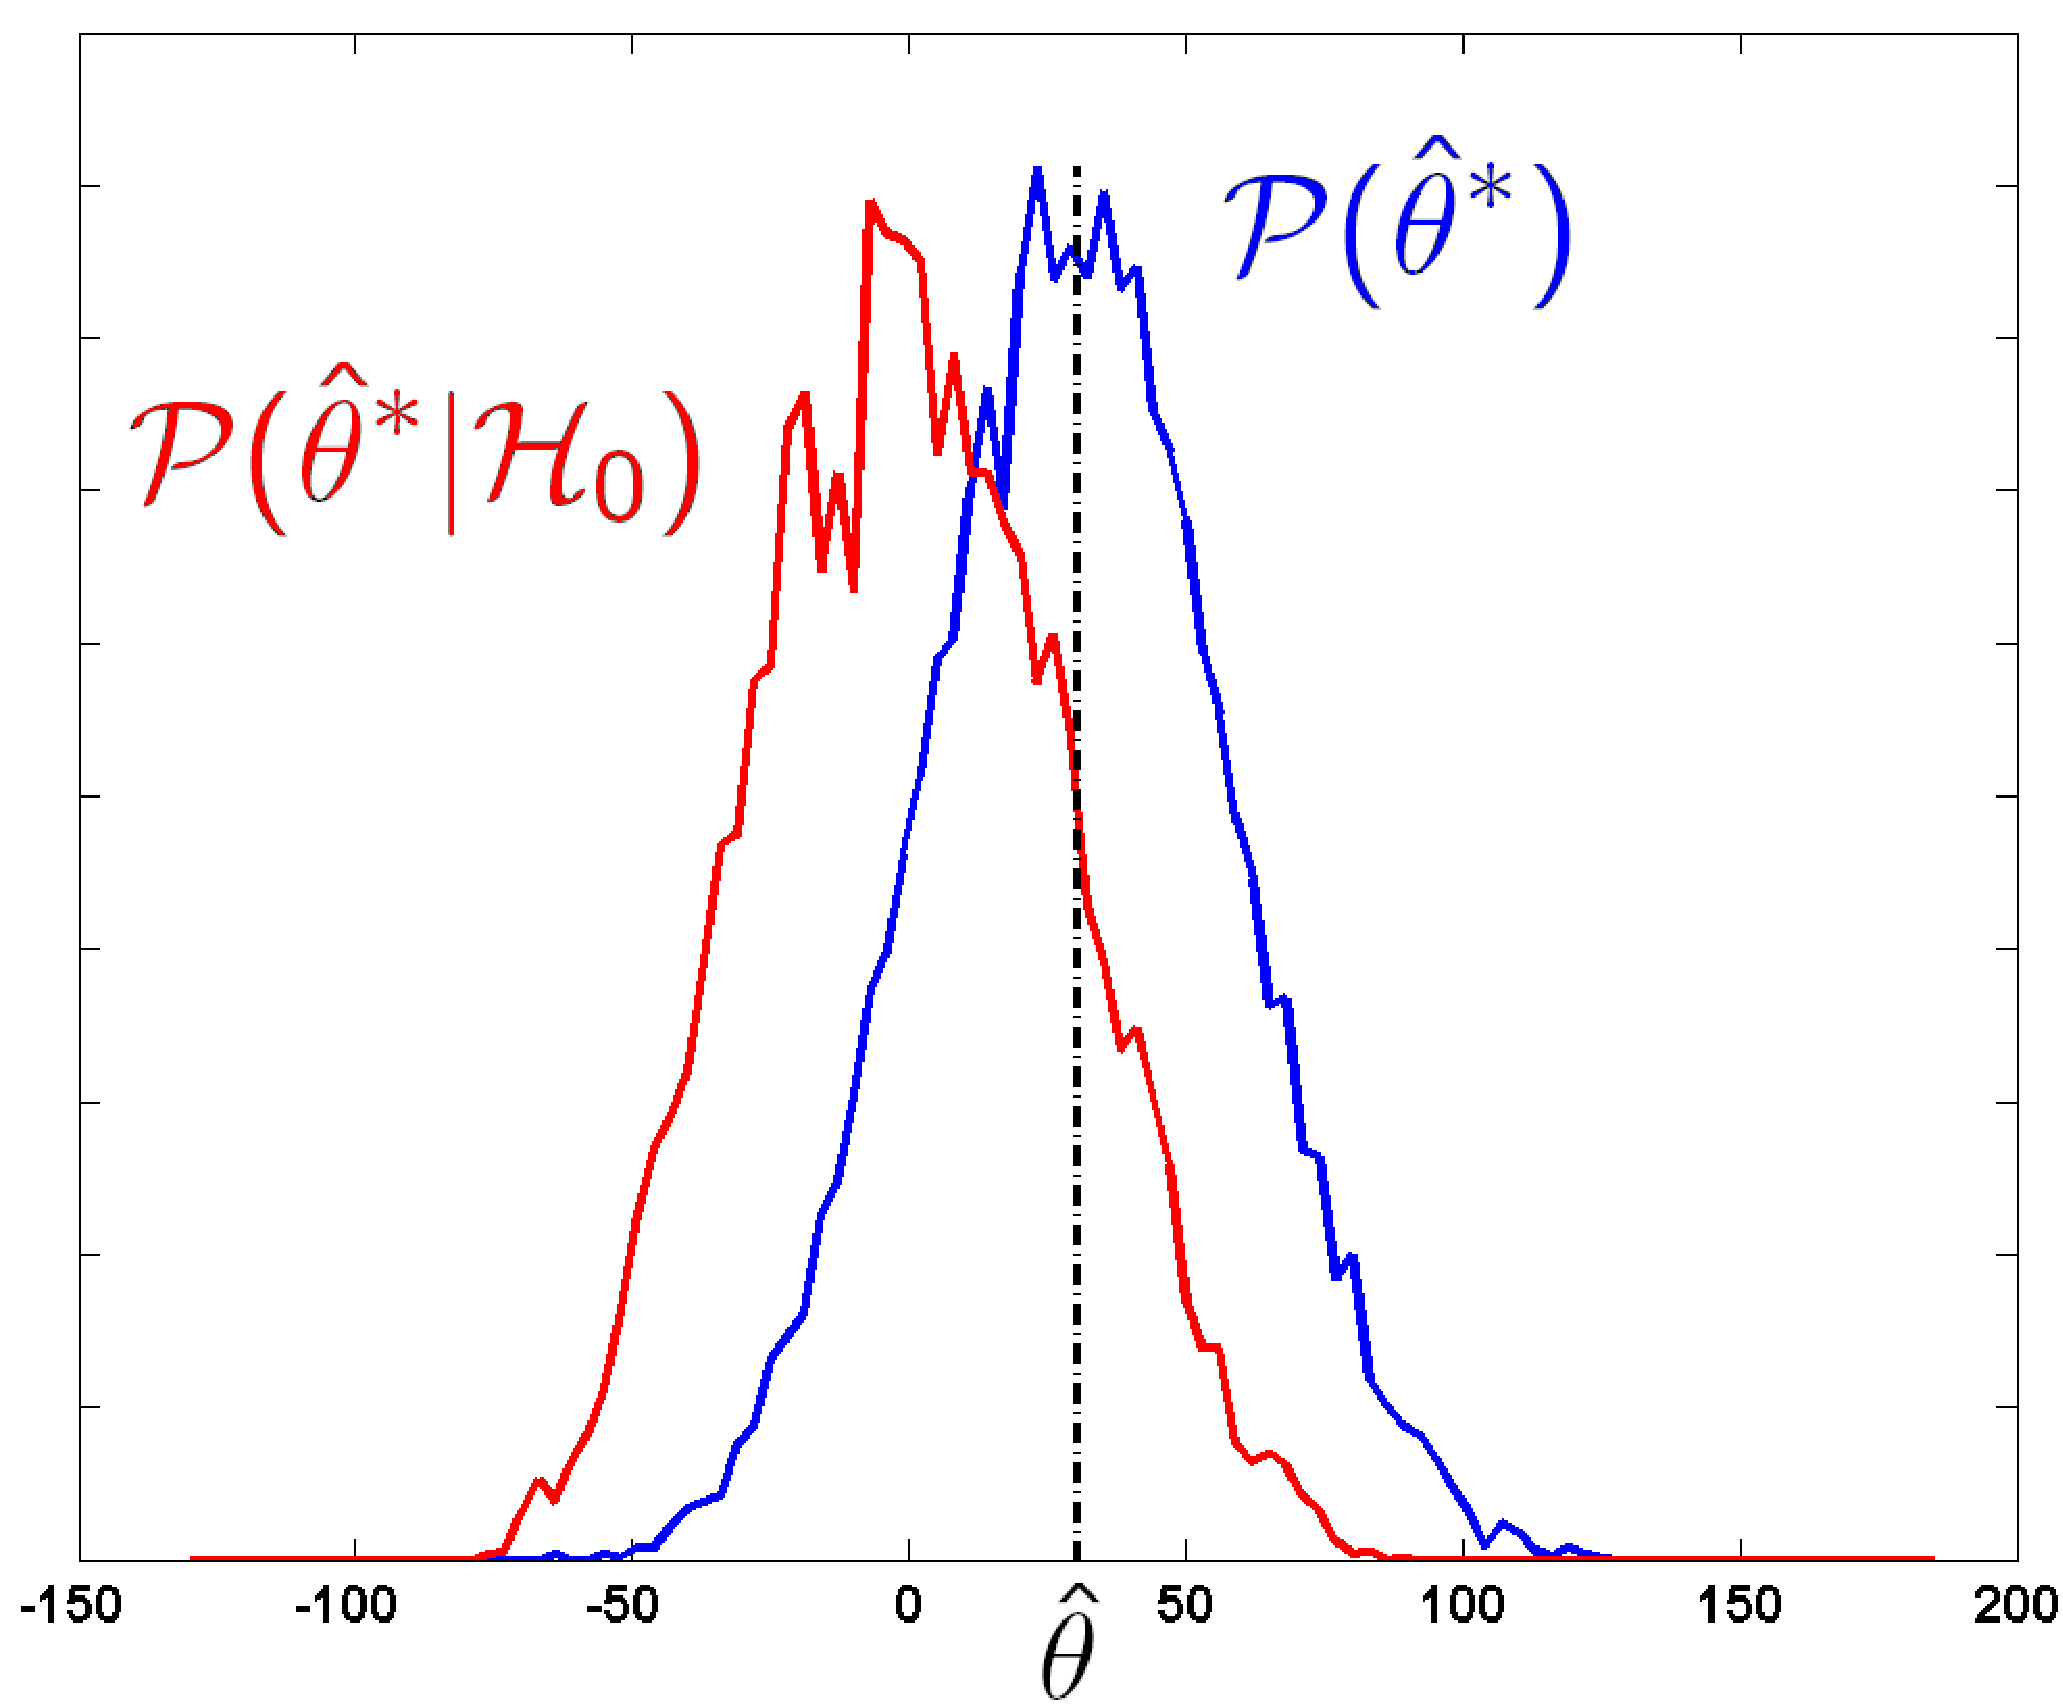
\includegraphics[scale=.2]{permboot}
\caption{Histograms of the bootstrap replications $\mathcal{P}(\hat{\theta}^{*})$ (blue), and the permutation replications $\mathcal{P}(\hat{\theta}^{*}|\mathcal{H}_{0})$ (red). }
\end{figure}
}
%%%%%%%%%%%%%%%%%%%%%%%%%%%%%%%%%%%%%%%%%%%%%%%%%
\frame
{
\frametitle{Remarks} 

\begin{itemize}

\item Permutation replications are computed  without replacement.

\

\item The  distribution of permutation replications approximates $\mathcal{P}(\theta^{*}|\mathcal{H}_0)$.

\

\item The bootstrap replications presented in the introduction are computed on resamples with replacements. The distribution of those bootstrap replications defines $\mathcal{P}(\theta^{*})$. 

\

\item Is there a way to get $\mathcal{P}(\theta^{*}|\mathcal{H}_0)$ using a bootstrap method ?

\end{itemize}

}


%%%%%%%%%%%%%%%%%%%%%%%%%%%%%%%%%%%%%%%%%%%%%%%%%
\frame
{
\frametitle{Computation of the two sample bootstrap test statistics}

\begin{beamercolorbox}[wd=\linewidth, rounded=true,shadow=true]{postit}

\begin{enumerate}
\item $\mathbf{x}=\lbrace \mathbf{x}_a;\mathbf{x}_b \rbrace$ of size $n+m=N$. 

\
\item Compute $B$ times:

\begin{itemize}
\item Bootstrap samples from  $\mathbf{x}$. Select the $n$ first values to define $\mathbf{x}^{*}_a$ and the last $m$ ones to define $\mathbf{x}^{*}_b$.

\

\item Compute the replications $\hat{\theta}^{*}(b)=\overline{x}_{a}^{*}-\overline{x}_{b}^{*}$
\end{itemize}

\item Approximate $\mathrm{ASL}_{boot}$ by:
$$
\widehat{\mathrm{ASL}}_{boot}= \frac{\# \lbrace \hat{\theta}^{*}(b) \geq \hat{\theta} \rbrace}{B}
$$
\end{enumerate}

\end{beamercolorbox}

}
%%%%%%%%%%%%%%%%%%%%%%%%%%%%%%%%%%%%%%%%%%%%%%%%%
\frame
{
\frametitle{Example on the mouse data}

\begin{figure}[!h]
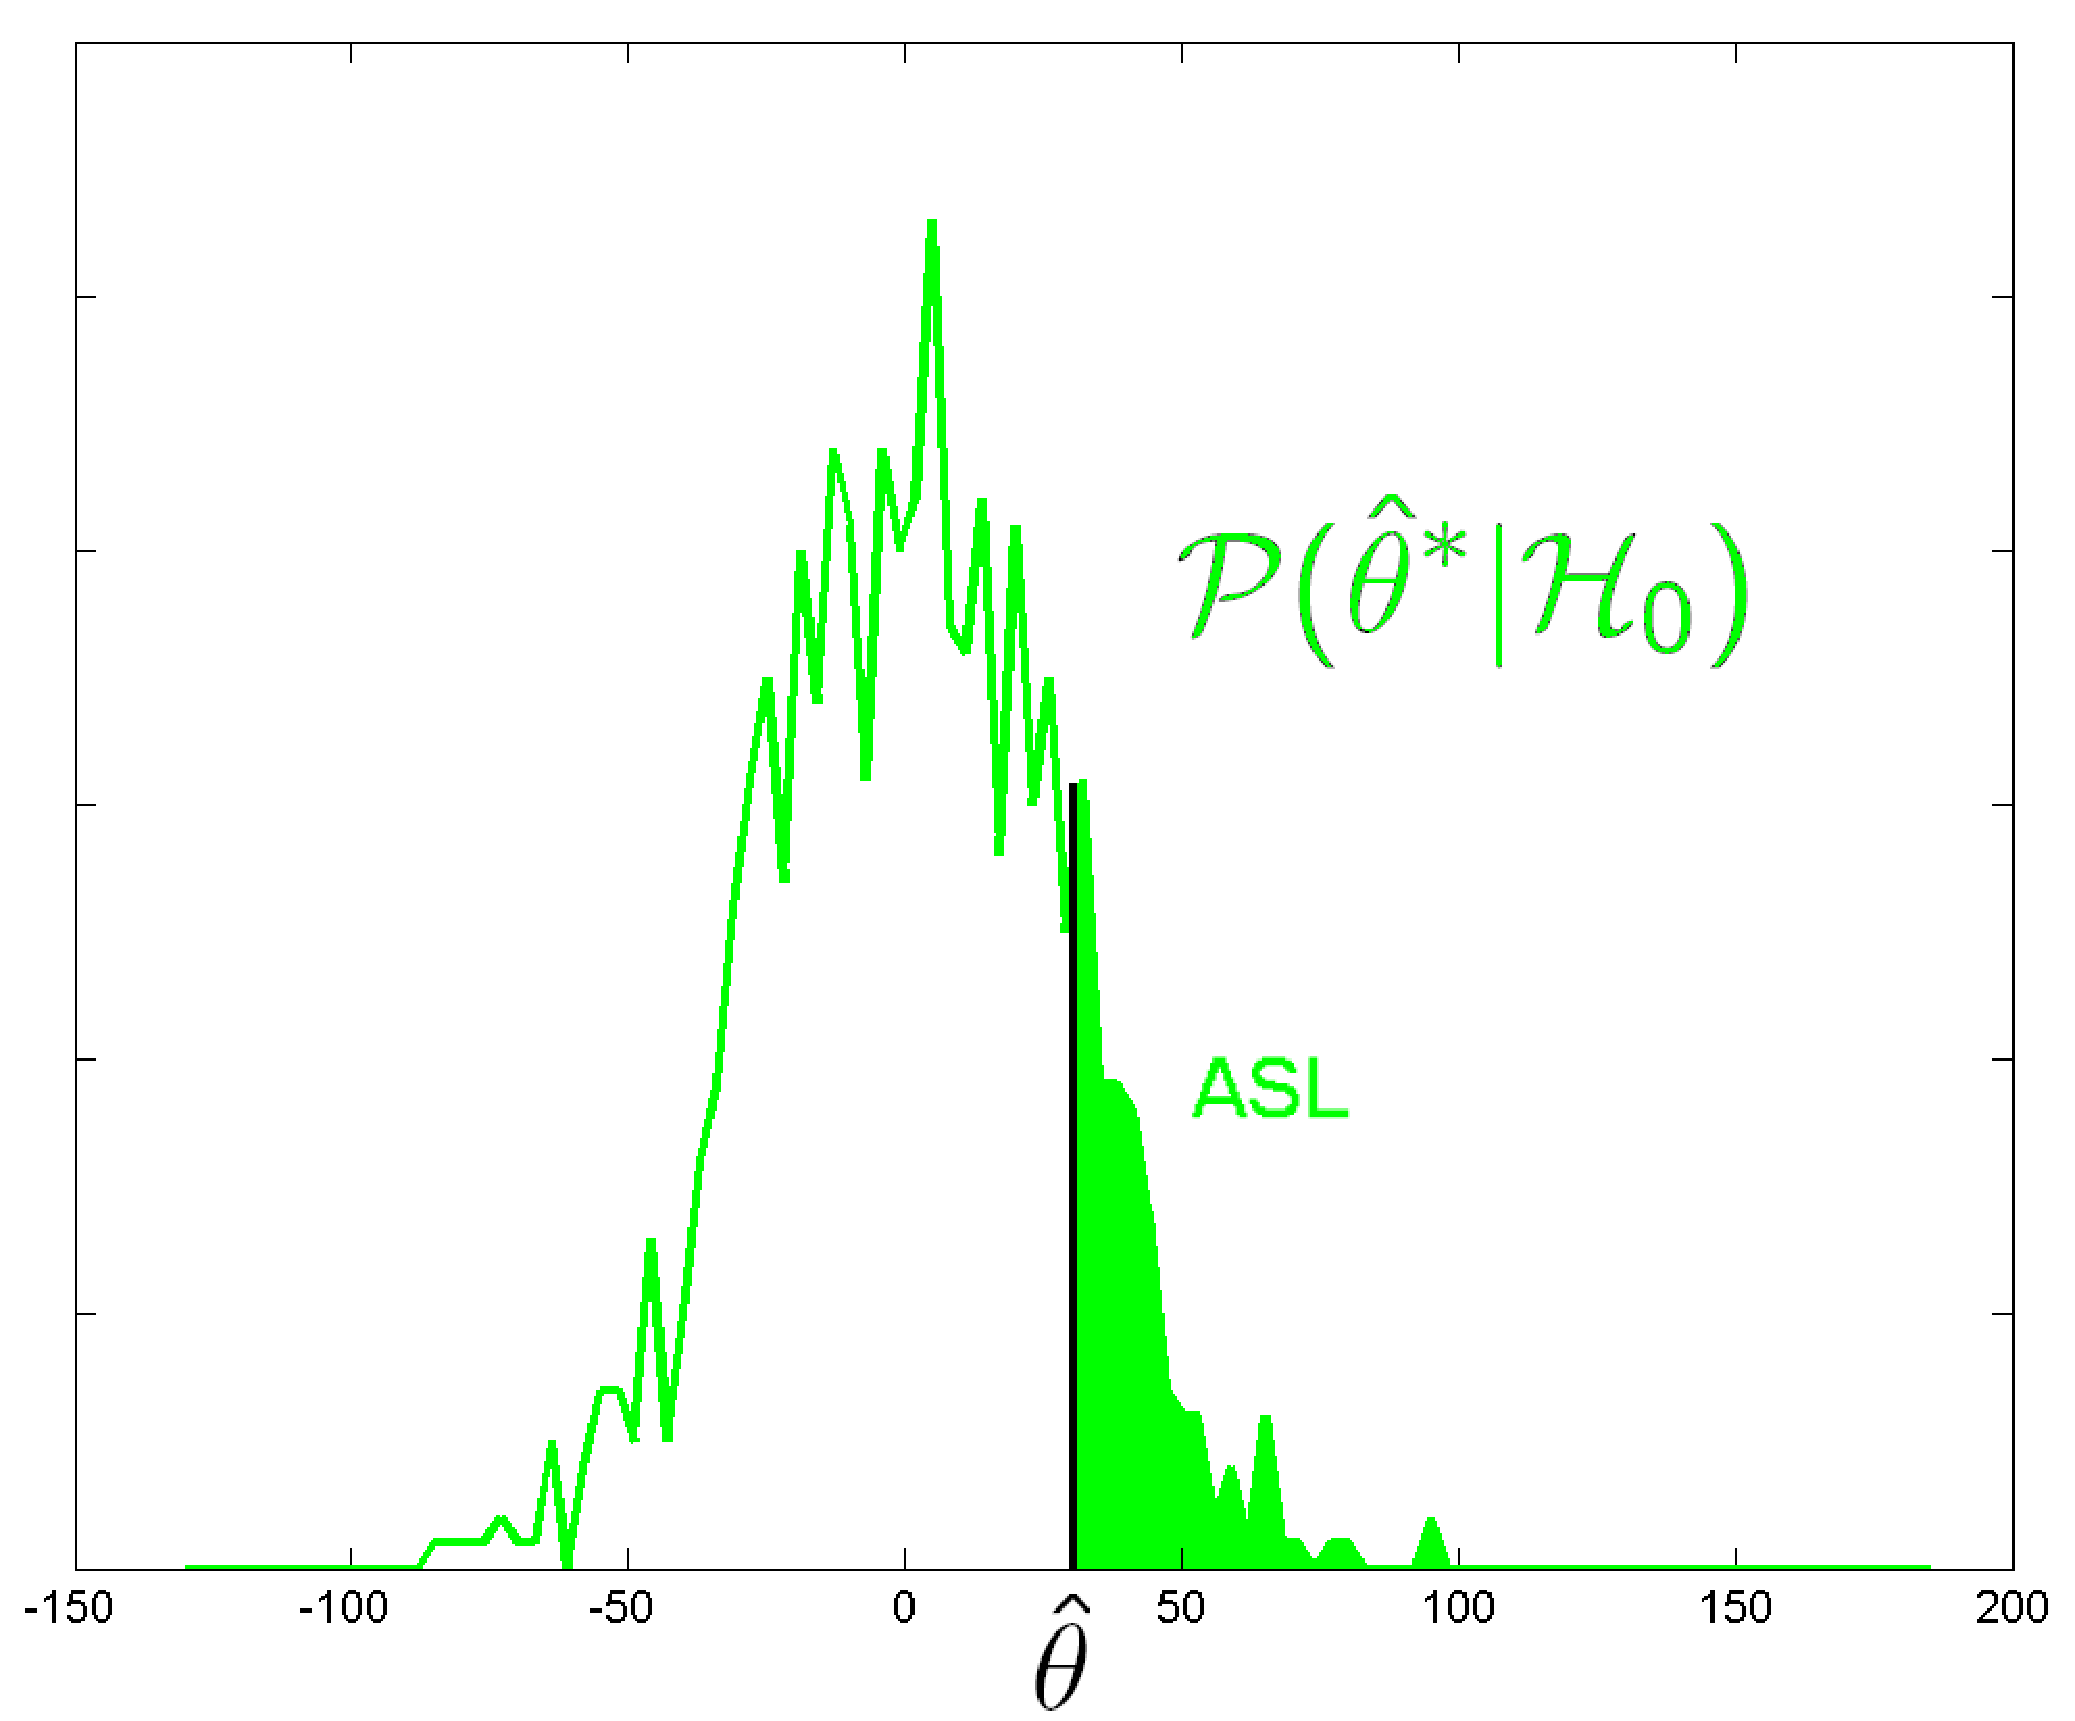
\includegraphics[scale=.2]{boot2sample}
\caption{Histogram of the \alert{bootstrap replications in the two sample test $\mathcal{P}(\hat{\theta}^{*}|\mathcal{H}_{0})$}. ASL is the green surface ($\mathrm{ASL}_{boot}=0.13$).}
\end{figure}

}

%%%%%%%%%%%%%%%%%%%%%%%%%%%%%%%%%%%%%%%%%%%%%%%%
\frame
{
\frametitle{Relationship between the permutation test and the bootstrap test}

\begin{itemize}
\item Very similar results in between the permutation test and the bootstrap test.


\


\item $\mathrm{ASL}_{perm}$ is the exact probability.   

\

\item $\mathrm{ASL}_{boot}$ is not an exact probability but is guaranteed to be accurate as an estimate of the ASL, as the sample size goes to infinity.

\

\item In the two-sample problem, the permutation test can  only test the null hypothesis $f_a=f_b$ while the bootstrap can perform other hypothesis testing.  


\end{itemize}

}




%%%%%%%%%%%%%%%%%%%%%%%%%%%%%%%%%%%%%%%%%%%%%%%%

\frame
{
\frametitle{Summary}

\begin{itemize}

\item Hypothesis testing has been introduced, involving the computation of a probability ASL

\

\item Permutation, Randomization  and bootstrap tests have been introduced as alternative to parametric tests.

\

\item Again the main difference in between those nonparametric tests, is the way the resamples are computed (with or without replacements).

\end{itemize}


}
